% chapters/chapter2/2_7_nmpc_design.tex
% !TeX root=../../main.tex

\section{طراحی کنترل‌کننده پیش‌بین مدل غیرخطی (\lr{NMPC})}
\label{sec:nmpc_design}

به‌منظور غلبه بر چالش‌های ناشی از دینامیک غیرخطی، اعمال قیود سخت فیزیکی و میراسازی فعال نوسانات بار، یک کنترل‌کننده پیش‌بین مدل غیرخطی (\lr{NMPC}) طراحی شده است. بر خلاف روش‌های کلاسیک که نیازمند خطی‌سازی حول نقطه تعادل هستند، این کنترل‌کننده با بهره‌گیری مستقیم از معادلات دیفرانسیل غیرخطی سیستم، رفتار آینده دینامیک را پیش‌بینی کرده و یک مسئله بهینه‌سازی مقید را در هر گام زمانی حل می‌کند.

برای فعال‌سازی قابلیت تغییر طول کابل به‌عنوان یک عملگر میراگر نوسان، بردار متغیرهای حالت از ۴ متغیر به ۶ متغیر بسط یافته است: $x = [x, \dot{x}, \theta, \dot{\theta}, l, \dot{l}]^T$. در این پیکربندی، ورودی‌های کنترلی مستقل سیستم شامل نیروی محرک کالسکه و شتاب کابل تعریف می‌شوند: $u = [F, \ddot{l}]^T$. انتخاب شتاب کابل ($\ddot{l}$) به‌عنوان متغیر دستکاری‌شونده، امکان استفاده از دو انتگرال‌گیر پیوسته برای استخراج یکپارچه سرعت ($\dot{l}$) و موقعیت کابل ($l$) را فراهم می‌آورد تا از بروز خطای کمبود مشتقات (\lr{Derivative Starvation}) در حل‌گرهای فیزیکی ممانعت شود.

\subsection{فرمولاسیون تابع هزینه و تنظیم افق‌های پیش‌بین}
استراتژی کنترل پیش‌بین بر پایه کمینه‌سازی یک تابع هزینه درجه دوم استوار است. زمان نمونه‌برداری سیستم $T_s = 0.05$ ثانیه تنظیم شده است. با توجه به پیچیدگی محاسباتی حل‌گرهای غیرخطی و محدودیت‌های پیاده‌سازی زمان‌درنگ (\lr{Real-time})، افق پیش‌بینی بر روی $N_p = 25$ تنظیم گردید که بازه زمانی $1.25$ ثانیه از آینده سیستم را پوشش می‌دهد. افق کنترلی نیز برای حفظ تعادل میان درجات آزادی بهینه‌ساز و بار محاسباتی، بر روی $N_c = 5$ تعیین شده است. فرمولاسیون تابع هزینه به‌صورت زیر است:
\begin{equation}
    \begin{split}
        J = & \sum_{i=1}^{N_p} e^T(k+i) Q e(k+i)                            \\
            & + \sum_{j=0}^{N_c-1} \Big[ u^T(k+j) R u(k+j)                  \\
            & \qquad\qquad + \Delta u^T(k+j) R_{\Delta} \Delta u(k+j) \Big]
    \end{split}
\end{equation}

ماتریس‌های وزنی به‌گونه‌ای تنظیم شده‌اند که علاوه بر حفظ تناسب پایه با کنترل‌کننده \lr{LQR}، ملاحظات عملیاتی عملگرها نیز رعایت شود:
\begin{itemize}
    \item \textbf{وزن خطای حالت ($Q$):} با ماتریس قطری $\text{diag}([1000, 10, 500, 10, 50, 10])$، بیشترین جریمه بر خطای موقعیت کالسکه ($1000$) و زاویه نوسان ($500$) اعمال شده است. دو درایه پایانی نیز وظیفه پایدارسازی سینماتیکی کابل را بر عهده دارند.
    \item \textbf{وزن تلاش کنترلی ($R$):} با تخصیص ماتریس $\text{diag}([1, 1])$، کمترین محدودیت بر دامنه مطلق عملگرها قرار داده شده است.
    \item \textbf{وزن نرخ تغییرات ورودی ($R_{\Delta}$):} برای جلوگیری از رفتار نامطلوب و نوسانی «بنگ-بنگ» و تضمین نرمی سیگنال‌های کنترلی، جریمه سنگینی به‌صورت $\text{diag}([50, 50])$ بر نرخ تغییرات نیرو و شتاب کابل اعمال شده است. این قید نرم از اعمال شوک‌های مکانیکی به سازه و استهلاک عملگرها جلوگیری می‌کند.
\end{itemize}

افزون بر تابع هزینه، رعایت قیود سخت فیزیکی (\lr{Hard Constraints}) در مسئله بهینه‌سازی اعمال شده است. این قیود شامل محدودیت نوسان آونگ در بازه $[-15^\circ, 15^\circ]$ (به‌فرم رادیان)، کران تغییرات طول کابل از $0.1$ تا $1.5$ متر، حداکثر نیروی کالسکه $50$ نیوتن و شتاب مجاز وینچ $5$ متر بر مجذور ثانیه است. جزئیات پیکربندی پارامترها و استخراج مدل افزوده دیفرانسیل در برنامه‌های \ref{code:nmpc_init} و \ref{code:nmpc_state} در پیوست \ref{app:matlab_codes} ارائه شده است.

\subsection{معماری حلقه کنترل}
به‌منظور استقرار الگوریتم در محیط شبیه‌سازی، معماری بلوک‌دیاگرام مطابق شکل \ref{fig:nmpc_block_diagram} توسعه یافته است. در این ساختار، کنترل‌کننده گسسته \lr{NMPC} در تعامل یکپارچه با مدل فیزیکی پیوسته قرار می‌گیرد.

\begin{figure}[ht]
    \centering
    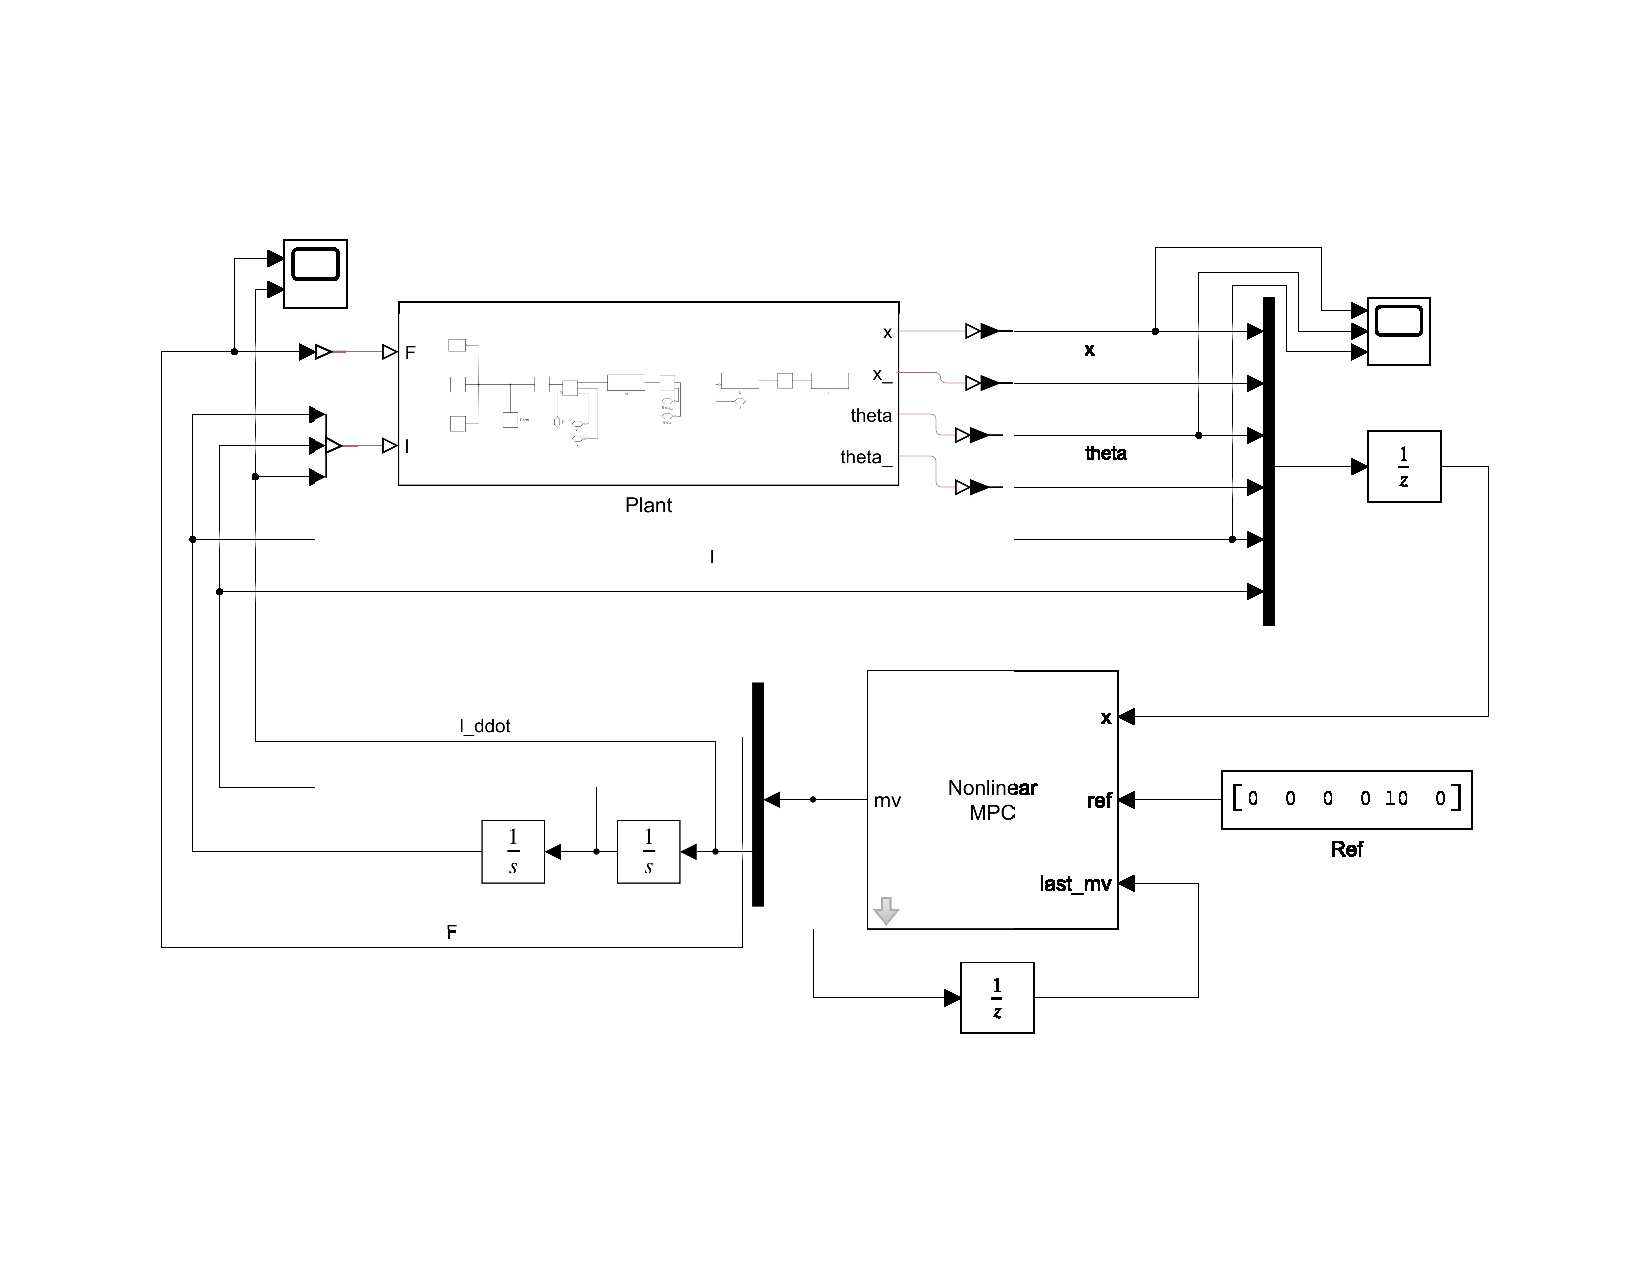
\includegraphics[width=\textwidth]{images/3_NMPC_Basic/MPC_block_diagram.pdf}
    \caption{\rl{معماری حلقه فیدبک کنترل‌کننده پیش‌بین غیرخطی و یکپارچه‌سازی سیگنال‌های سینماتیکی.}}
    \label{fig:nmpc_block_diagram}
\end{figure}

همان‌گونه که در دیاگرام ساختاری نمایان است، سیگنال شتاب کابل پس از عبور از زنجیره انتگرال‌گیرها، متغیرهای سینماتیکی را تولید کرده و به‌صورت بازخورد هم‌زمان به همراه حالات اصلی به کنترل‌کننده تزریق می‌شود. به‌منظور رفع مشکل حلقه‌های جبری (\lr{Algebraic Loops}) ناشی از وابستگی مستقیم خروجی به ورودی در یک گام زمانی، از یک بلوک تأخیر واحد ($1/z$) با شرایط اولیه منطبق بر وضعیت فیزیکی آغازین سیستم ($[x_0, 0, \theta_0, 0, l_0, 0]$) در مسیر بازخورد استفاده شده است. این معماری مداربسته، شالوده اصلی ارزیابی‌های دینامیکی در فصل نتایج خواهد بود.